\section{Design and Implementation}
% General
% Describe how you have chosen to solve the problem
% Argue clearly for the choices made when designing and developing the solution.
The primary tool used for solving the problem of finding candidates of plagiarised documents has been the LSH algorithm and data structure. LSH has been chosen as it is an efficient and space efficient algorithm which makes it ideal to perform a nearest neighbour search. Combined with other techniques, which will be described in the following, have laid the foundation of the solution.

\subsection{Modules}
% Introduce section
In this section will the designed and implemented Python modules be introduced, as well as reasoning for why certain design choices were made.

\paragraph{Wikiparser}
% Binary search to find location of article in index file.
% Decision to unzip small amount and process at a time.
% Remind what the size of the decompressed data is as a motivation to decompress on-the-fly
The \emph{Wikipedia} database is provided as a compressed archive of articles in the open-source \emph{bzip2} format with an accompanied index file listing the contents of the archive. Because the articles are formatted in XML and wikitext\footnote{A special markup language used by Wikipedia to format plain text into articles} the space of the compressed archive is significantly reduced. Because of the sheer amount of data, decompressing and keeping every article in memory is simply infeasible. Remember that the archive is 16 GB compressed and 55 GB decompressed. We have circumvented this issue by performing an on-the-fly, as-needed decompression of articles while they are fed to the LSH algorithm. This reduces the necessary amount of memory to only keeping a block (100 articles) in memory at a time. This operation is performed by reading the index file line by line, in which the start and end position of the data block can be found, then seeking and reading that block in the compressed archive file, decompressing and parsing the XML structure to separate articles. The implementation is achieved by overriding the \texttt{\_\_iter\_\_} and \texttt{\_\_next\_\_} methods from the \emph{Python} programming language to create an iterable object.

Another much needed functionality is fast lookup of articles. This is desirable because we quickly want to retrieve articles which has been marked as plagiarised. Because we have no intend to decompress the article archive and waste hard drive space, we want to perform the decompression on-the-fly. Since the index file is ordered by the article id we can perform binary search and find the requested article in $\log(u)$ time. Although this binary search is mostly trivial, we have to take special care when seeking in the file since the position of file pointer is not guaranteed to be placed at the start of a new line. Following the binary search we can decompress the block and parse the XML as before.

\paragraph{LSH}
% The report does not discuss the benefits and downsides of LHS and what they mean for this project (compared documents have to be similar in length for it to detect candidates i.e).

% Argue for the choice of parameters like q, r, b, k....
The LSH algorithm has a few different parameters, that should be set according to what you wish to achieve. One of them is the size of the shingles, $q$. For the matching of whole documents $q = 9$, as it is considered safe for large documents.\cite{leskovec2014mining} % Write something about the value of q for matching paragraphs
The remaining two parameters are $b$ and $r$, which is the number of bands and the number of rows in each band respectively. Choosing these parameters, will change the probability of the signatures in our data structure of becoming a candidate. With $b=20$ and $r=5$ we get the following curve as seen in figure~\ref{fig:lsh}. This gives us that when the similarity of two documents are $0.51$, then the probability of becoming a candidate is $>1/2$.

\begin{figure}[h]
	\centering
    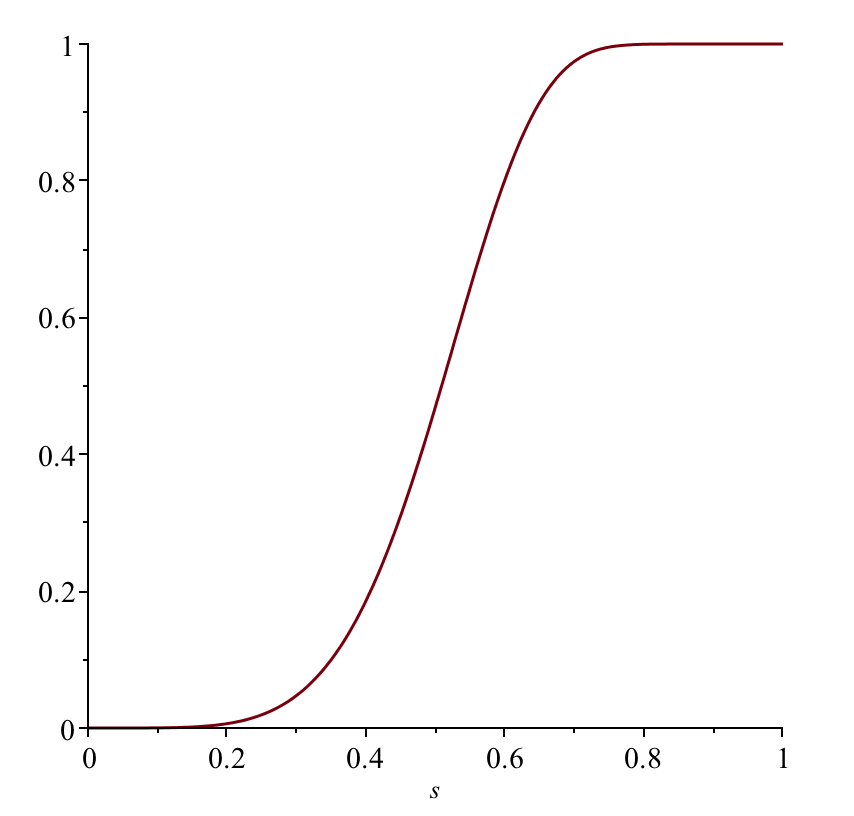
\includegraphics[width = 0.4\linewidth]{docs/report/input/lsh.png}
    \captionsetup{width = \linewidth}
    \caption{Probability of becoming a candidate versus Jaccard similarity of documents of choices of $b=20$ and $r=5$, $1-(1-s^r)^b$}
    \label{fig:lsh}
\end{figure}

\paragraph{Database}
% Show design of tables
% Argue why a database was used
% in Table 2 you have the same doc_id twice with different id. Is this the intended design?
Although LSH is a space efficient data structure and algorithm there is a trade-off between space and accuracy. Hashing many documents will inevitably grow beyond the amount what can be stored in memory. Storing the LSH data structure on disk will incur a performance penalty but will enable the data structure to grow in order of magnitudes larger than what we can fit in memory. We have chosen a database management system, specifically \emph{SQLite}, to store the LSH data structure. This is a nice abstraction because we can rely on the database for performance and optimisation of the queries. The design of the database schemes can be seen in table~\ref{table:sqlite1} and~\ref{table:sqlite2} and is comprised of two tables \emph{hashes} and \emph{documents} in which the attribute \emph{id} in \emph{documents} is a foreign key referencing the \emph{hashes} table. This allows the database to only store the LSH band once and associate multiple documents to that band.

To assist with lookup performance both tables have indices on critical attributes. The \emph{hashes} table has a combined index on the \emph{hash, band} attributes while the \emph{documents} table has an index on the the \emph{id} attribute alone. This is useful because an usual operation is the check, whether and band is already stored in the database, so as to only store it once. Both tables has a set of constraints such that no two identical bands can be stored and no article can be added to the same band twice, since this information is redundant.

% http://www.roman10.net/2018/04/10/visualize-sqlite-database-schema/

\begin{table}[ht]
    \begin{minipage}[b]{0.56\linewidth}
        \centering
        \begin{tabular}{|l|l|l|}
            \hline
            id (int) & hash (bytes{[}4{]}) & band (int) \\ \hline
            0        & 0xa3f723e8          & 1          \\ \hline
            1        & 0x21be6122          & 1          \\ \hline
            2        & 0xc945e851          & 2          \\ \hline
        \end{tabular}
        \caption{Table \emph{hashes} which stores information on each LSH band with the hash value and the band id}
        \label{table:sqlite1}
    \end{minipage}\hfill
    \begin{minipage}[b]{0.4\linewidth}
        \centering
        \begin{tabular}{|l|l|}
            \hline
            id (int) & doc\_id (int) \\ \hline
            0        & 22            \\ \hline
            1        & 29            \\ \hline
            2        & 22            \\ \hline
        \end{tabular}
        \caption{Table \emph{documents} which associates documents with LSH bands from table \emph{hashes}}
        \label{table:sqlite2}
    \end{minipage}
\end{table}

\paragraph{MapReduce} TODO

\begin{figure}[h]
	\centering
    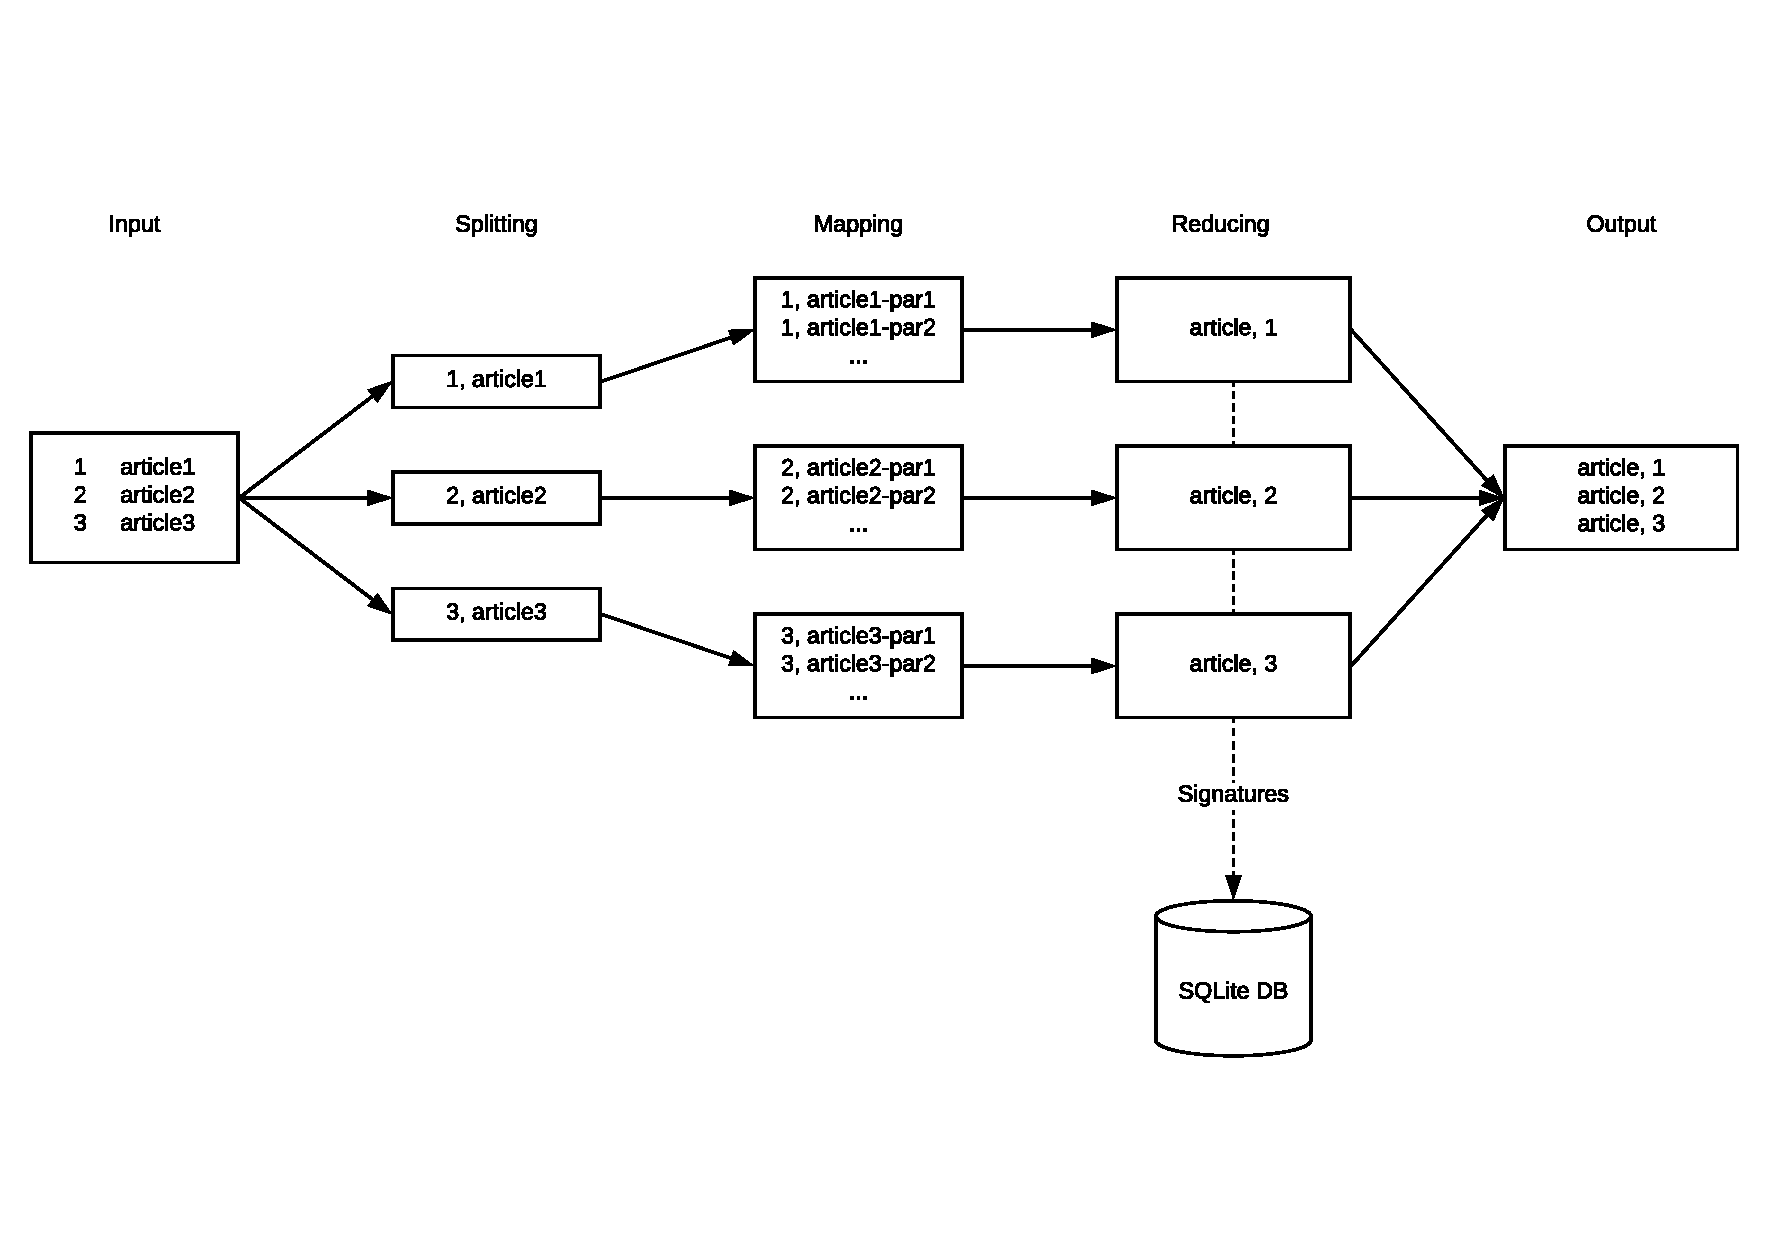
\includegraphics[width = \linewidth]{docs/report/input/mapreduce.pdf}
    \captionsetup{width = \linewidth}
    \caption{UPDATE ME!}
    \label{fig:mapreduce}
\end{figure}

\subsection{Data processing}
\subsubsection{Generate}
\label{sec:gen}

% http://citeseerx.ist.psu.edu/viewdoc/download?doi=10.1.1.458.9440&rep=rep1&type=pdf

% Insert flow figure of generate
\begin{figure}[ht]
	\centering
    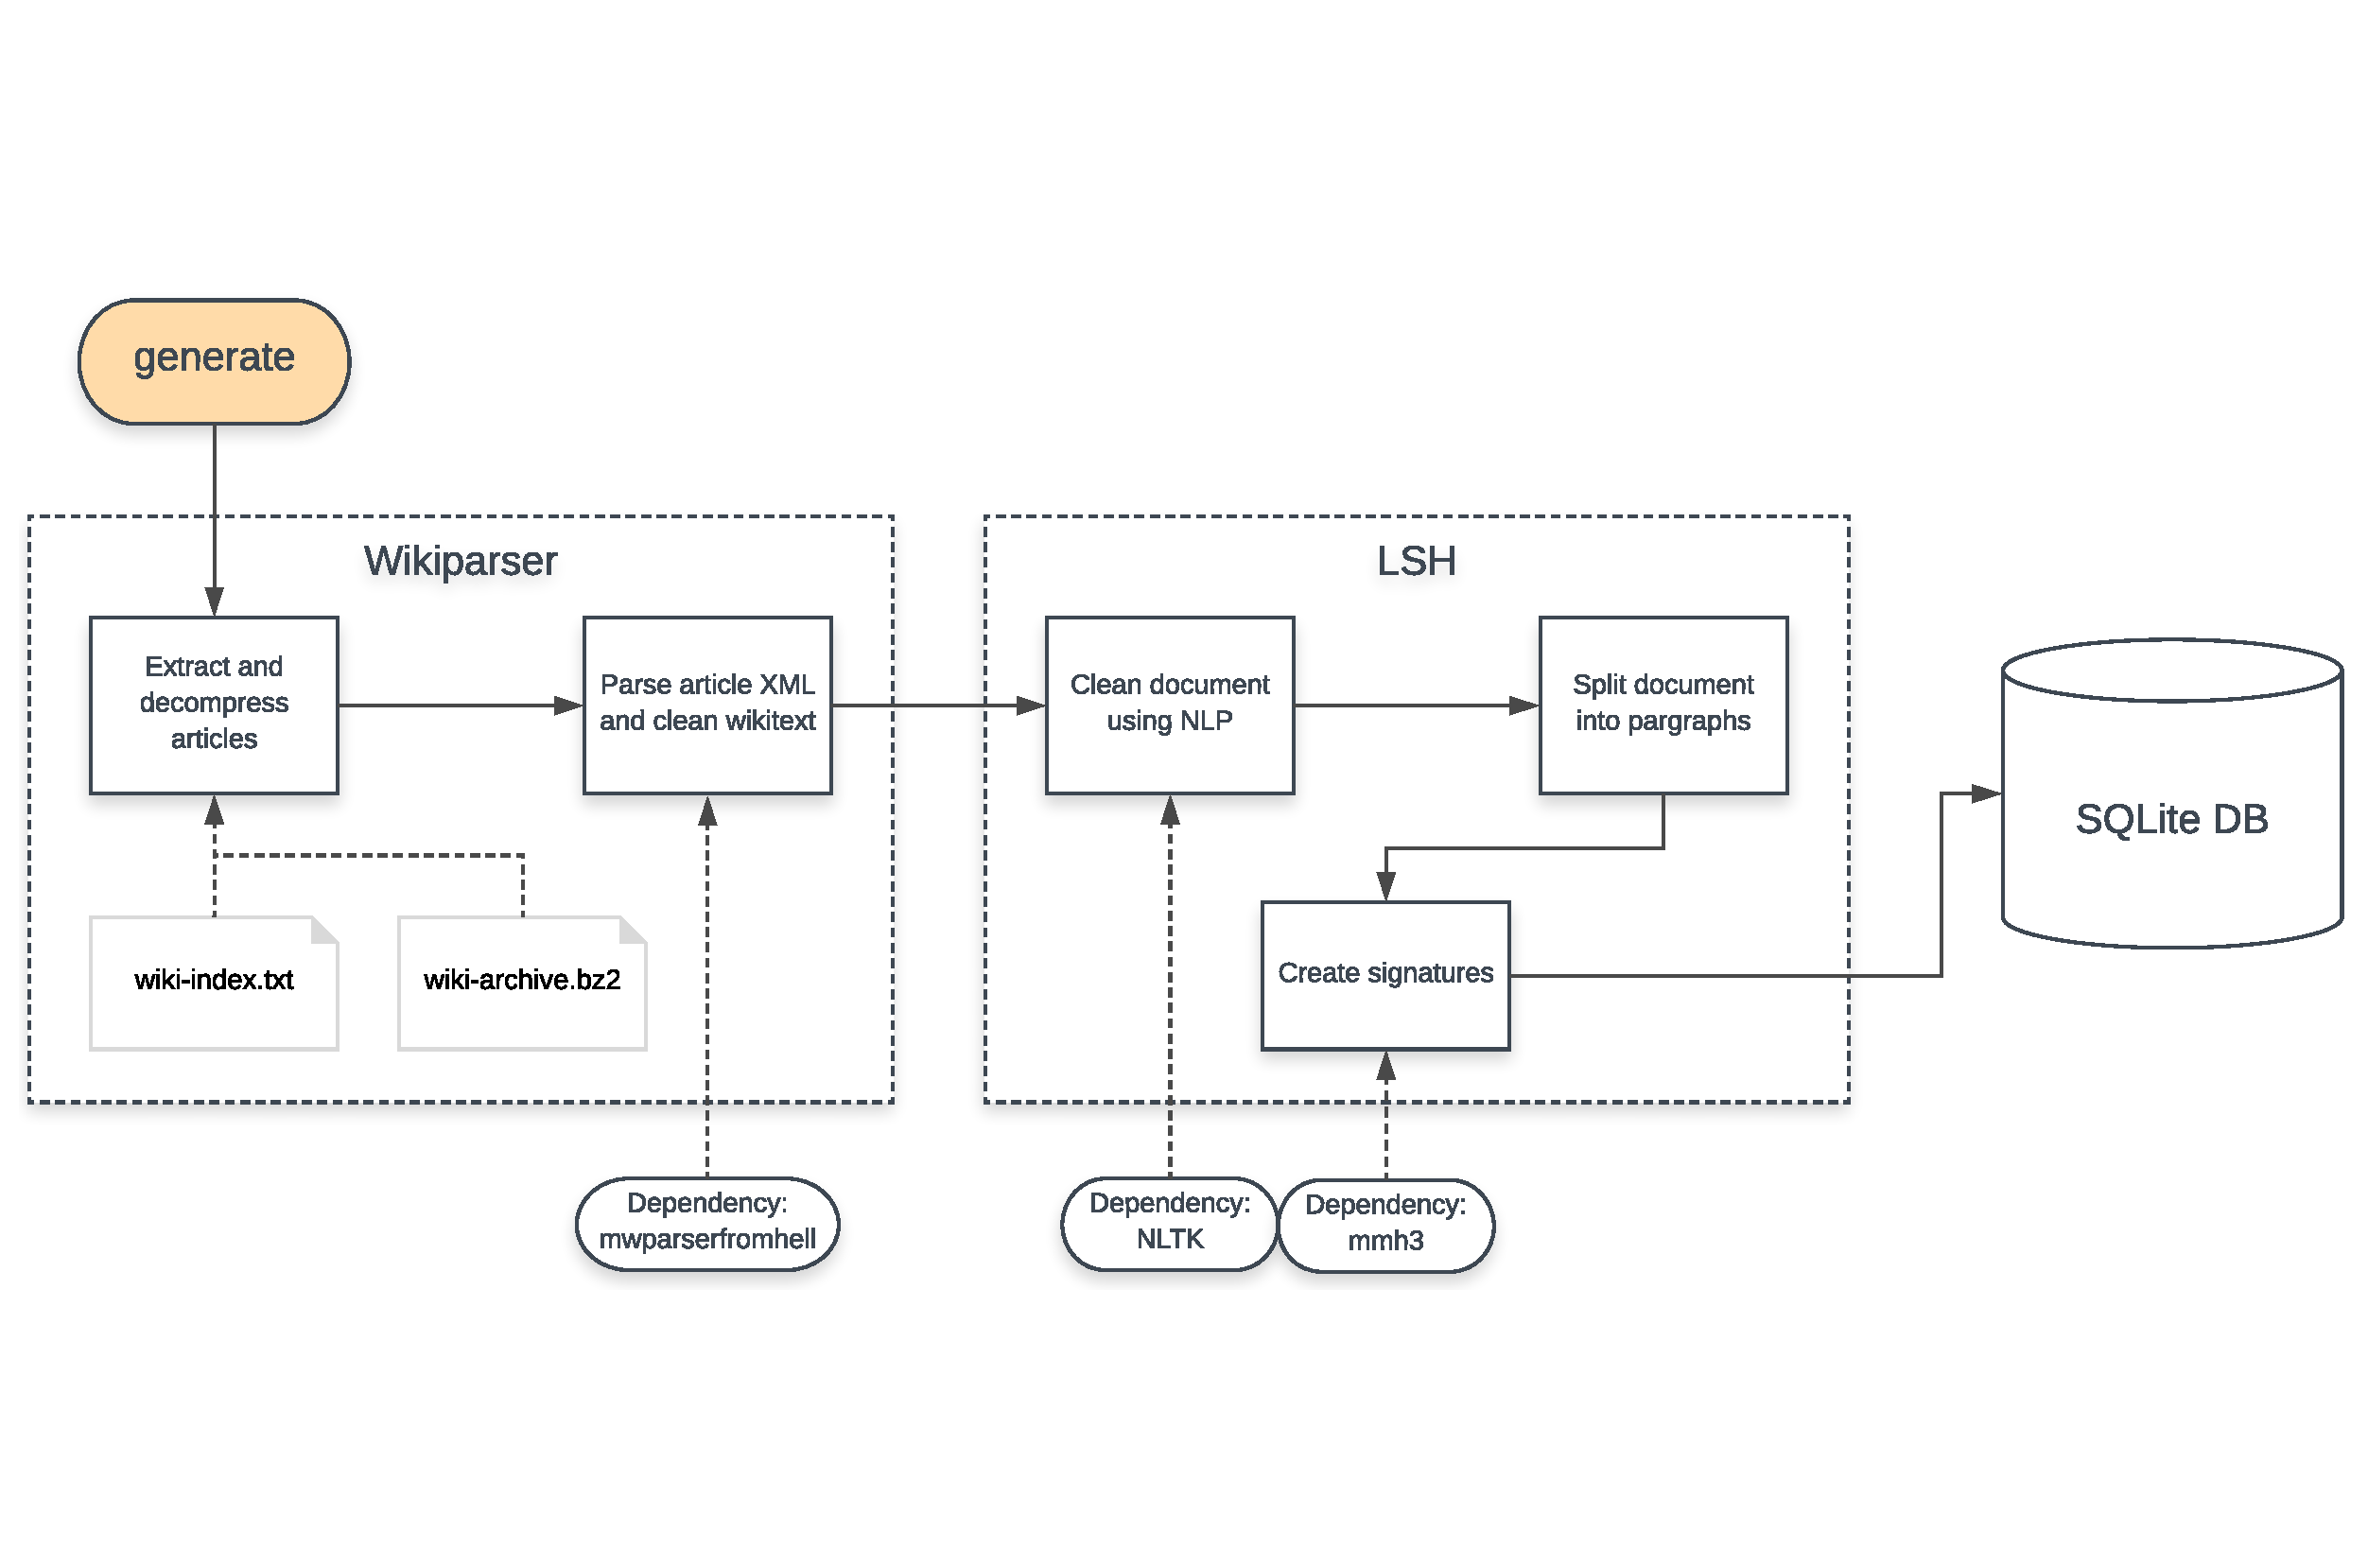
\includegraphics[width = \linewidth]{docs/report/input/generate.pdf}
    \captionsetup{width = \linewidth}
    \caption{UPDATE ME!}
    \label{fig:generate}
\end{figure}

\begin{description}
    \item[Extract and decompress articles] The Wikiparser will extract and decompress the articles. This will either be every Wikipedia article or a limited amount, depending on the given program arguments.
    \item[Parse article XML and clean wikitext] Each decompressed Wikipedia article will have the content of its text field in the XML parsed and striped of the wikitext.
    \item[Lowercase everything] To prepare the content of the article to have stop words removed, is everything transformed to lowercase.
    \item[Remove stop words] To make the solution more robust against plagiarised content where minor changes has been made all stop words are removed. Consider the following two sentences where a single word has changed: \say{This is \emph{a} test senctence of nine words total}, \say{This is \emph{the} test sentence of nine words total}. Hashing these two sentences will generate completely different hash values, but it is clear that they should be marked as plagiarised. This is avoided by removing the stop words as defined by NLTK\footnote{\url{https://gist.github.com/sebleier/554280}} and using the NLTK library\footnote{\url{https://www.nltk.org}}. Removing the stop words reduce both of them to \say{test shingle nine words total}. The reduced sentences will now produce the same hash value and be detected as plagiarised correctly.
    \item[Remove special characters] As with stop words, where a small change in a sentence will result in a completely different hash value, will the inclusion of special characters like \say{.}, \say{,}, \say{;} etc. give a completely different hash value. E.g is the hash value of \say{example,} not equal to the hash value of \say{example}. For this reason are all special characters removed from the content.
    \item[Replace all whitespace] To avoid creating shingles with the \emph{empty string}, when passing the content to the LSH algorithm, are all whitespace characters\footnote{\url{https://en.wikipedia.org/wiki/Whitespace_character}} replaced with a single space. As the content of the article is split by any whitespace character, then would consecutive whitespace characters result in the empty string being added to the shingle. Furthermore is it not sufficient to simply split by the space character without removing the remaining whitespace characters, as they would then be part of the words after the split and thereby having an influence on the generated hash value.
    \item[Split document into paragraphs] The document is then split into paragraphs of 80 words. A paragraph is considered to be around 125 words\footnote{\url{https://wordcounter.net/blog/2017/01/23/102485_how-many-paragraphs-is-1000-words.html}} but empirical data showed that removing stop words reduced the words in an article to $63\%$, which give $125 \cdot 0.63 \approx 80$. Each paragraph will overlap the previous paragraph by $50\%$. The reason being that if was not done, then would an adversary be able to place its plagiarised paragraph such that would only have a $50\%$ overlap with paragraph in the data structure. This means that the similarity of the adversary's paragraph with the data structure's will be at most $0.5$ and from \ref{fig:lsh} one can that the probability of being chosen as a candidate is approximately $50\%$. Having each paragraph overlap the previous one in the data structure will increase the similarity to $0.75$ which increases the probability to approximately $1$.
    \item[Create and store signatures in database] Each paragraph for each article is then passed to the LSH algorithm, which will generate the signature and store it in the database.
\end{description}

\subsubsection{Lookup}

% Insert flow figure of lookup
\begin{figure}[ht]
	\centering
    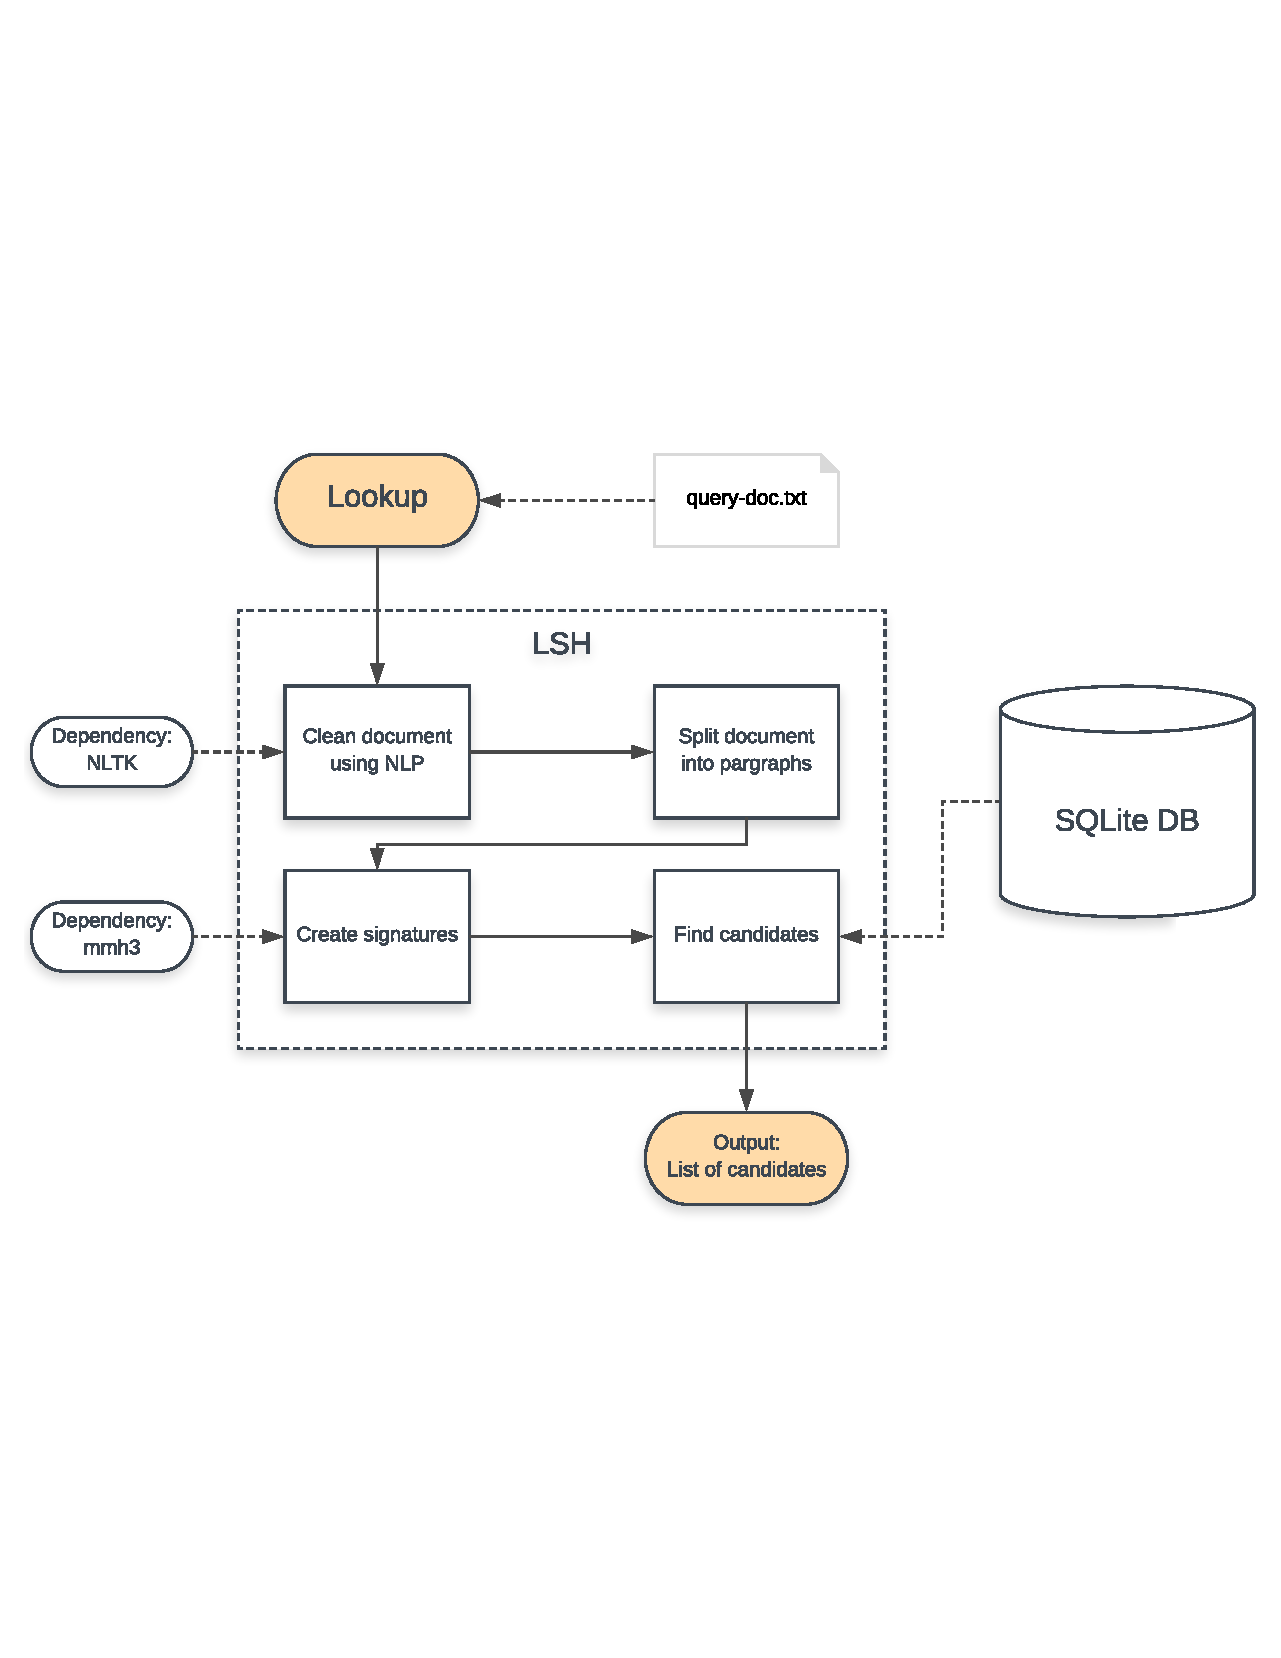
\includegraphics[width = \linewidth]{docs/report/input/lookup.pdf}
    \captionsetup{width = \linewidth}
    \caption{UPDATE ME!}
    \label{fig:lookup}
\end{figure}

% Are you comparing a given document to every single article in the wiki database?
\begin{description}
    \item[Prepare query document] The query document is prepared before the signature is generated by the LSH algorithm just like the articles were in the \emph{generate} process described in section~\ref{sec:gen}. That includes lowercase everything, remove stop words, remove special characters, replace all whitespace characters with a space character and splitting the document into paragraphs of the same size as the was used during the \emph{generate} process.
    \item[Create signatures] When the preparation of the data content is complete is the signature of the document generated, using the same LSH configuration as was used when generating the database.
    \item[Lookups in database to find candidates] The generated signature is then used to find matches for in the database. If a match is found, is the article ID and appended to a list. When all candidates are found is the list returned to the user.
\end{description}